\documentclass[dvipsnames]{article}
\input tmp.inputs
\pagestyle{empty}
\usepackage[]{xcolor}
\usepackage{tikz}
\usetikzlibrary{shapes,arrows,chains}

\begin{document}
%	\begin{tikzpicture} 
%	\umlsimpleclass[x=0,y=0]{Human}
%	\umlsimpleclass[x=10,y=0]{Pet}
%	\umlassoc[mult1=1, mult2=1..*, pos1=0.1, pos2=0.9, name=owns]{Human}{Pet}
%	\node[above] at (owns-1) {owns};
%	\end{tikzpicture}
%	\begin{tikzpicture}
%	\umlsimpleclass[x=0,y=4]{DSView}
%	\umlclass[x=0,y=0]{DSCluster}{
%	- int : numRobot\\
%	- DSQueryRobot[] : activeQueries\\
%	- int : numHost}{ 
%	+ StartNewComputation()\\
%	+ MakeMove()\\
%	+ RetryQuery()\\
%}
%	\umlclass[x=4,y=-5]{DSClusterInterface - Actor}{
%	- int : host\\
%	- int : numRobot
%}{}
%
%	\umlclass[x=10,y=-0]{DSRobot - Actor}{
%	- String : myNode\\
%	- DSGraph : myView\\
%	- ActorRef[] : activeQueryChecker
%}{}
%
%	\umlclass[x=10,y=-5]{DSQueryChecker - Actor}{
%	- String : myNode\\
%	- DSGraph : myView\\
%	- DSQuery: query
%}{}
%\umluniassoc[name=hasDSView]{DSCluster}{DSView}
%\node[left] at (hasDSView-1) {has};
%
%\umldep[name=depDSRobot]{DSCluster}{DSRobot - Actor}
%\node[above] at (depDSRobot-1) {Create};
%\node[below] at (depDSRobot-1) {actorSystemInitialization};
%
%
%\umldep[name=depQueryChecker]{DSRobot - Actor}{DSQueryChecker - Actor}
%\node[right] at (depQueryChecker-1) {Create};
%
%\umldep[geometry=|-, name=depClusterInterface]{DSCluster}{DSClusterInterface - Actor}
%\node[right] at (-3,-3) {ConnectNewHost};
%
%\umldep[geometry=-|, name=depClusterInterface]{DSCluster}{DSClusterInterface - Actor}
%
%
%
%\umluniassoc[geometry=|-|,name=hasDSCluster]{DSClusterInterface - Actor}{DSCluster}
%\node[right, align=left] at (hasDSCluster-1) {(Static access to\\ host instance)};
%
%
%	\end{tikzpicture}
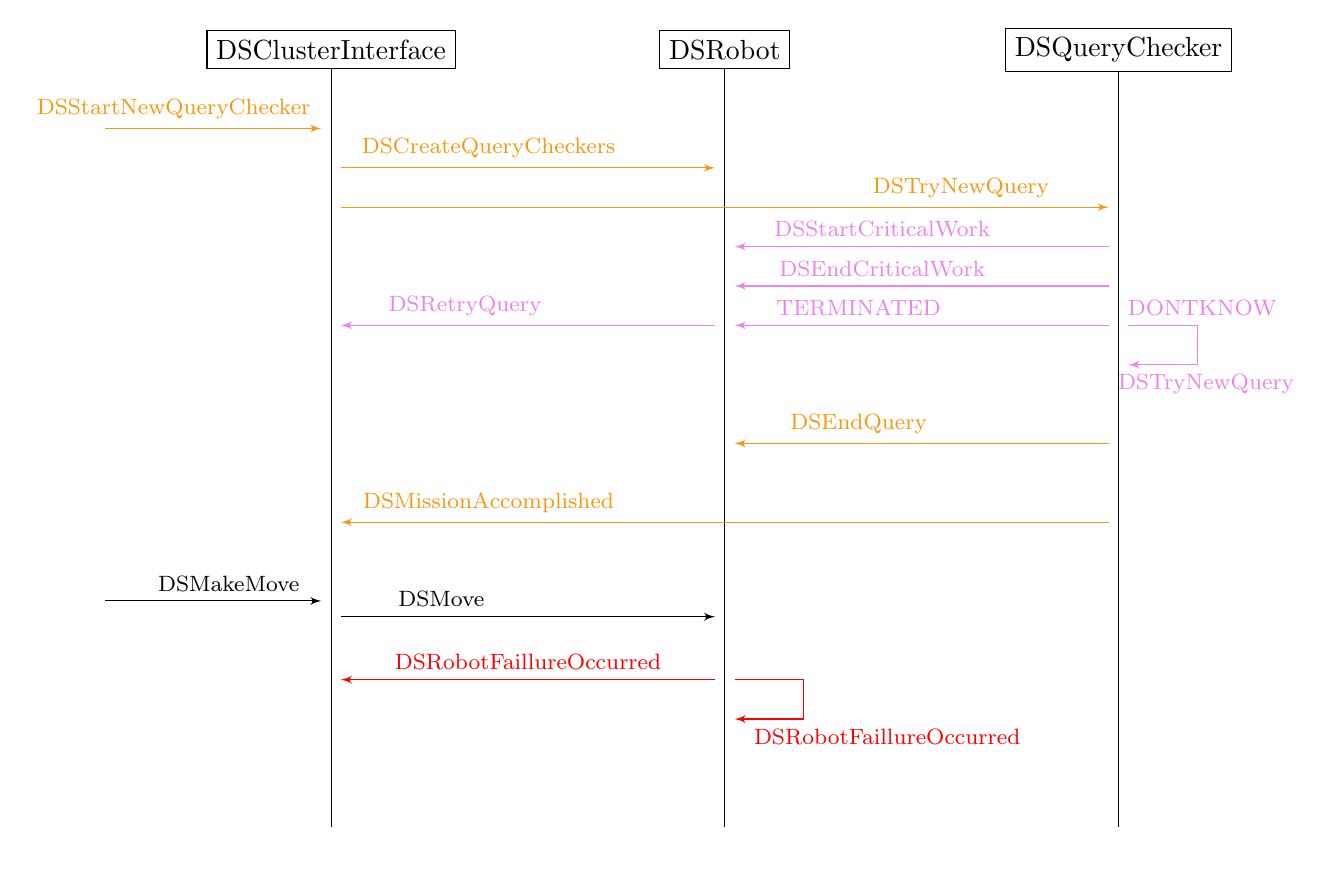
\begin{tikzpicture}
\node[draw] at (0, 0)   (topA) {DSClusterInterface};
\node[draw] at (5, 0)   (topB) {DSRobot};
\node[draw] at (10, 0)   (topC) {DSQueryChecker};
\node[] at (-3,-1) (unoA) {};
\node[] at(0,-1)(unoB){};

\node[] at (0,-1.5) (dueA) {};
\node[] at(5,-1.5)(dueB){};

\node[] at (0,-2) (treA) {};
\node[] at(10,-2)(treB){};

\node[] at (10,-2.5) (quattroA) {};
\node[] at(5,-2.5)(quattroB){};

\node[] at (10,-3) (cinqueA) {};
\node[] at(5,-3)(cinqueB){};

\node[] at (10,-3.5) (seiA) {};
\node[] at(5,-3.5)(seiB){};

\node[] at (5,-3.5) (setteA) {};
\node[] at(0,-3.5)(setteB){};

\node[] at (10,-3.5) (ottoA) {};
\node[] at(10,-4)(ottoB){};

\node[] at (10,-5) (noveA) {};
\node[] at(5,-5)(noveB){};

\node[] at (10,-6) (dieciA) {};
\node[] at(0,-6)(dieciB){};

\node[] at (-3,-7) (undiciA) {};
\node[] at(0,-7)(undiciB){};

\node[] at (0,-7.2) (dodiciA) {};
\node[] at(5,-7.2)(dodiciB){};

\node[] at (5,-8) (trediciA) {};
\node[] at(0,-8)(trediciB){};

\node[] at (5,-8) (quattordiciA) {};
\node[] at(5,-8.5)(quattordiciB){};


\node[] at (0, -10)   (bottomA) {};
\node[] at (5, -10)   (bottomB) {};
\node[] at (10, -10)   (bottomC){};

\draw[] (topA) -- (bottomA);
\draw[] (topB) -- (bottomB);
\draw[] (topC) -- (bottomC);

\draw[-latex', YellowOrange](unoA) node[above,xshift=1cm] {\footnotesize{DSStartNewQueryChecker}} -- (unoB);

\draw[-latex', YellowOrange](dueA) node[above,xshift=2cm] {\footnotesize{DSCreateQueryCheckers}} -- (dueB);
\draw[-latex', YellowOrange](treA) node[above,xshift=8cm] {\footnotesize{DSTryNewQuery}} -- (treB);

\draw[-latex', Violet](quattroA) node[above,xshift=-3cm] {\footnotesize{DSStartCriticalWork}} -- (quattroB);

\draw[-latex', Violet](cinqueA) node[above,xshift=-3cm] {\footnotesize{DSEndCriticalWork}} -- (cinqueB);

\draw[-latex', Violet](seiA) node[above,xshift=-3.3cm] {\footnotesize{TERMINATED}} -- (seiB);

\draw[-latex', Violet](setteA) node[above,xshift=-3.3cm] {\footnotesize{DSRetryQuery}} -- (setteB);

\draw[-latex', Violet](ottoA) -- node[below,yshift=-0.5cm,xshift=0.5cm] {\footnotesize{\ DSTryNewQuery}} node[above,xshift=0.5cm] {\footnotesize{DONTKNOW}}++ (1,0) |- (ottoB) ;

\draw[-latex', YellowOrange](noveA) node[above,xshift=-3.3cm] {\footnotesize{DSEndQuery}} -- (noveB);

\draw[-latex', YellowOrange](dieciA) node[above,xshift=-8.0cm] {\footnotesize{DSMissionAccomplished}} -- (dieciB);

\draw[-latex', Black](undiciA) node[above,xshift=1.7cm] {\footnotesize{DSMakeMove}} -- (undiciB);

\draw[-latex', Black](dodiciA) node[above,xshift=1.4cm] {\footnotesize{DSMove}} -- (dodiciB);

\draw[-latex', Red](trediciA) node[above,xshift=-2.5cm] {\footnotesize{DSRobotFaillureOccurred}} -- (trediciB);

\draw[-latex', Red](quattordiciA) -- node[below,yshift=-0.5cm,xshift=1.5cm] {\footnotesize{DSRobotFaillureOccurred}} ++ (1,0) |- (quattordiciB) ;

\end{tikzpicture}

\end{document}